\documentclass[12pt,a4paper]{article}
\usepackage[utf8]{inputenc}
\usepackage{amsmath}
\usepackage[labelfont=bf]{caption}
\usepackage{amsfonts}
\usepackage{amssymb}
\usepackage{graphicx}
\usepackage{fourier}
\usepackage[left=2cm,right=2cm,top=2cm,bottom=2cm]{geometry}
\author{Devin Cody}
\begin{document}


\begin{figure}
\centering
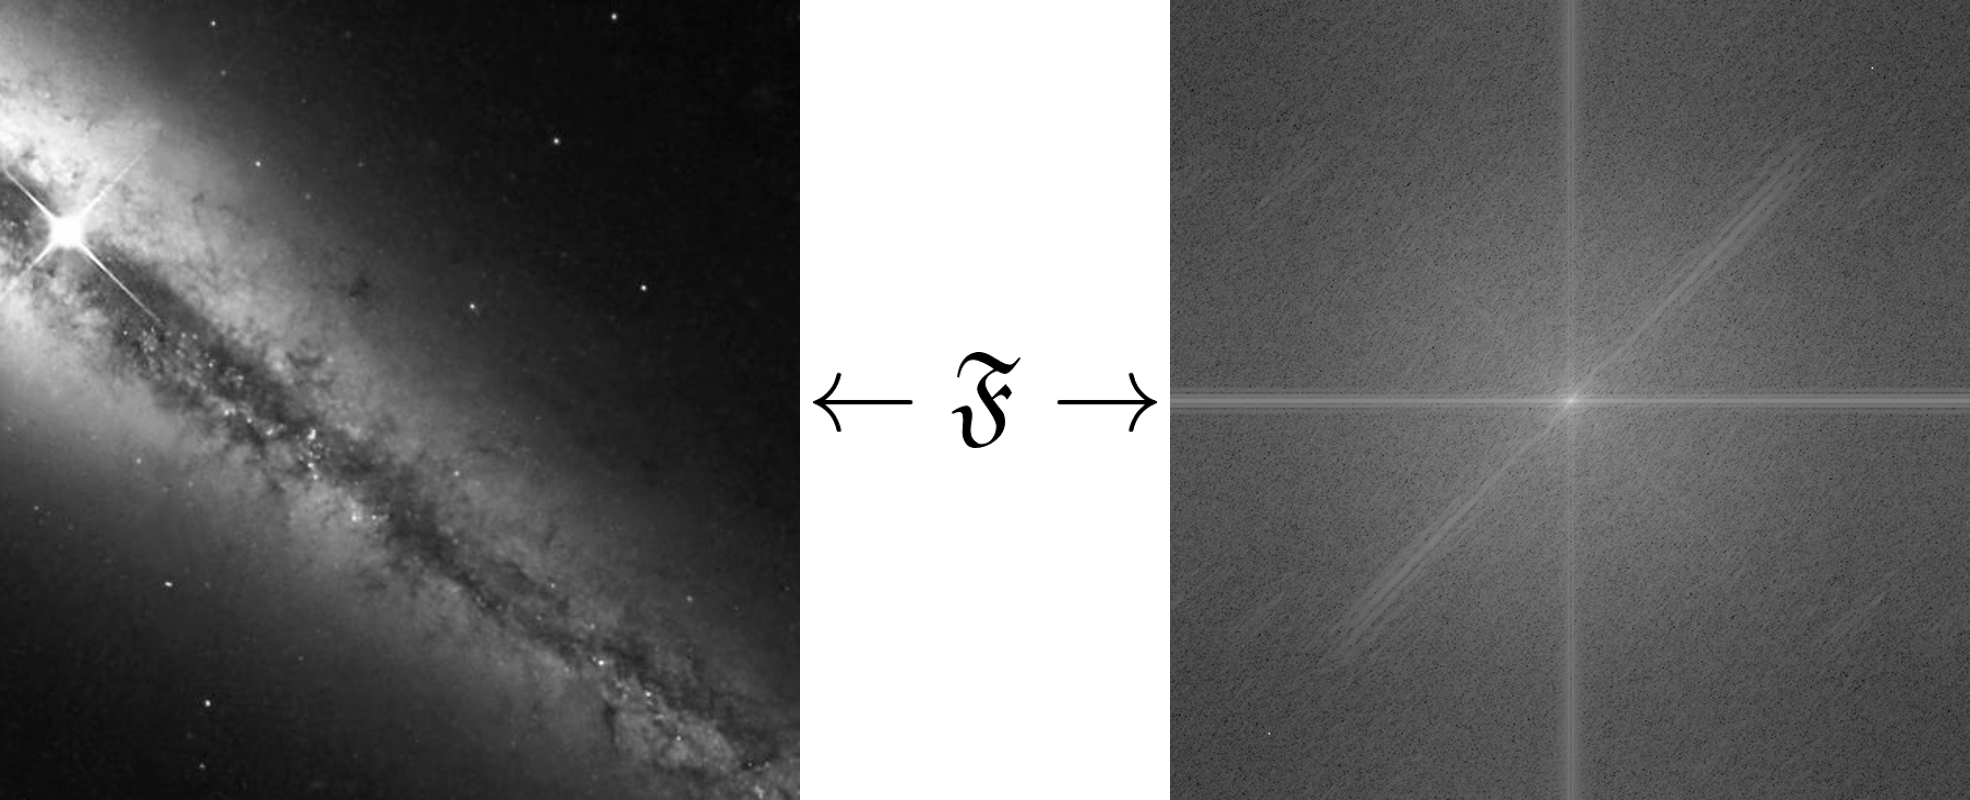
\includegraphics[width=\textwidth]{_images/FT.png}
\caption{\textbf{Galaxy in ``image domain'' (left) and ``Fourier domain'' (right) |} Comparison of the ``Traditional'' depiction of a galaxy in the ``image'' domain (Left) and an equally-valid depiction of the same galaxy in “Fourier” domain (Right). The script F denotes that these two images are related by the Fourier Transform.}
\end{figure}


\begin{figure}
\centering
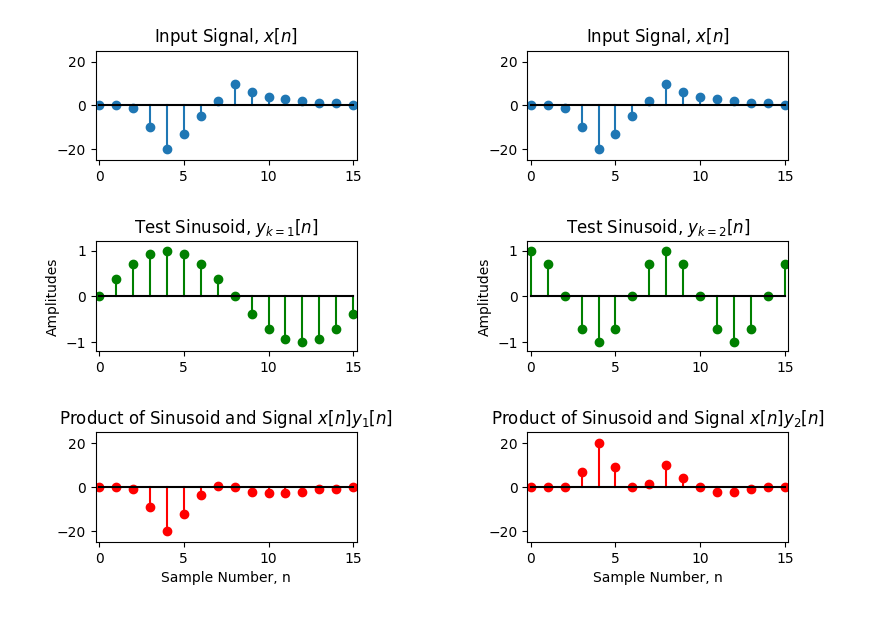
\includegraphics[width=\textwidth]{_images/FourierCorrelation3-m56p3-47p1.png}
\caption{\textbf{Correlation of an input signal (top) and two sinusoids (middle) |} On the left, we show the result of correlating a particular input signal with a cosine wave with period 16. For correlation, each sample in the input signal is multiplied by the corresponding sample in the test sinusoid. The result of this multiplication is shown on the bottom in red. To complete the correlation, we simply sum across all the points in the red signal. On the right, the same input signal is correlated with another cosine, this time with a period of 8. Again, the element-wise multiplication of the two signals is shown on the bottom in red. For the Fourier transform, the input signal is correlated against 16 total sinusoids (8 sines and 8 cosines). The mathematics of the Fourier Transform are shown in equation ****}
\end{figure}



\begin{figure}
\centering
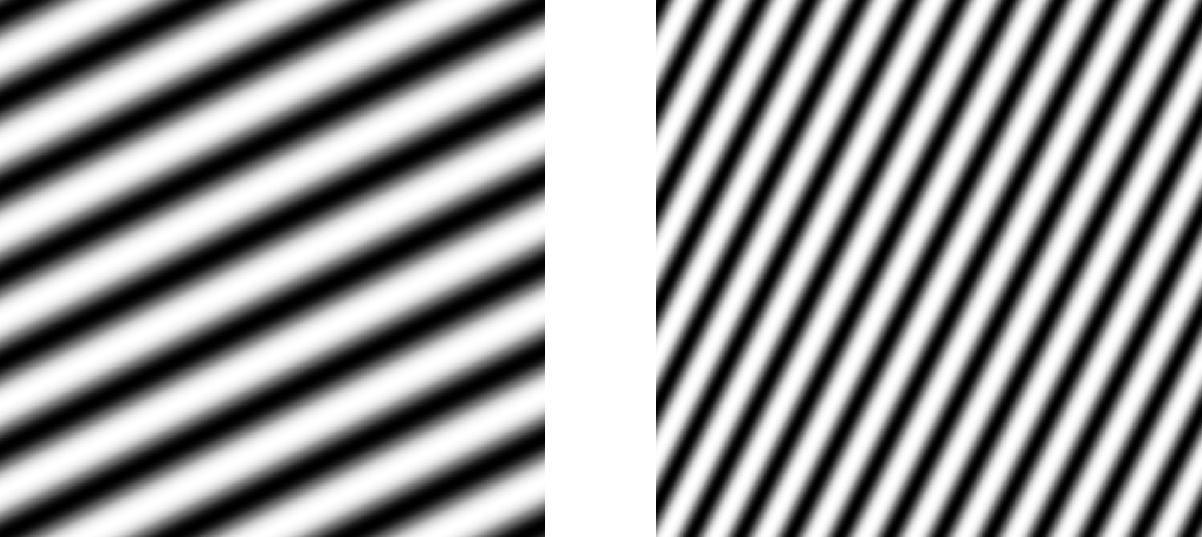
\includegraphics[width=\textwidth]{_images/TwoTestSinusoids.png}
\caption{\textbf{ Examples of two-dimensional test sinusoids |} Whereas the one-dimensional Fourier transform used one-dimensional test sinusoids, the two-dimensional Fourier transform uses two-dimensional test sinusoids. Here are two potential test sinusoids that might be used on a 1024x1024 grid. While the one-dimensional Fourier transform needed N+2 sinusoids, the two-dimensional Fourier transform needs N+2xN+2 test sinusoids. Each one of these N+2xN+2 sinusoids has its own direction and frequency. As shown, the two sinusoids have different ``directions'' and frequencies. Furthermore, the sinusoids have different phases, the image on the left was generated with cosines and the image on the right was generated with sines.}
\end{figure}


\begin{figure}
\centering
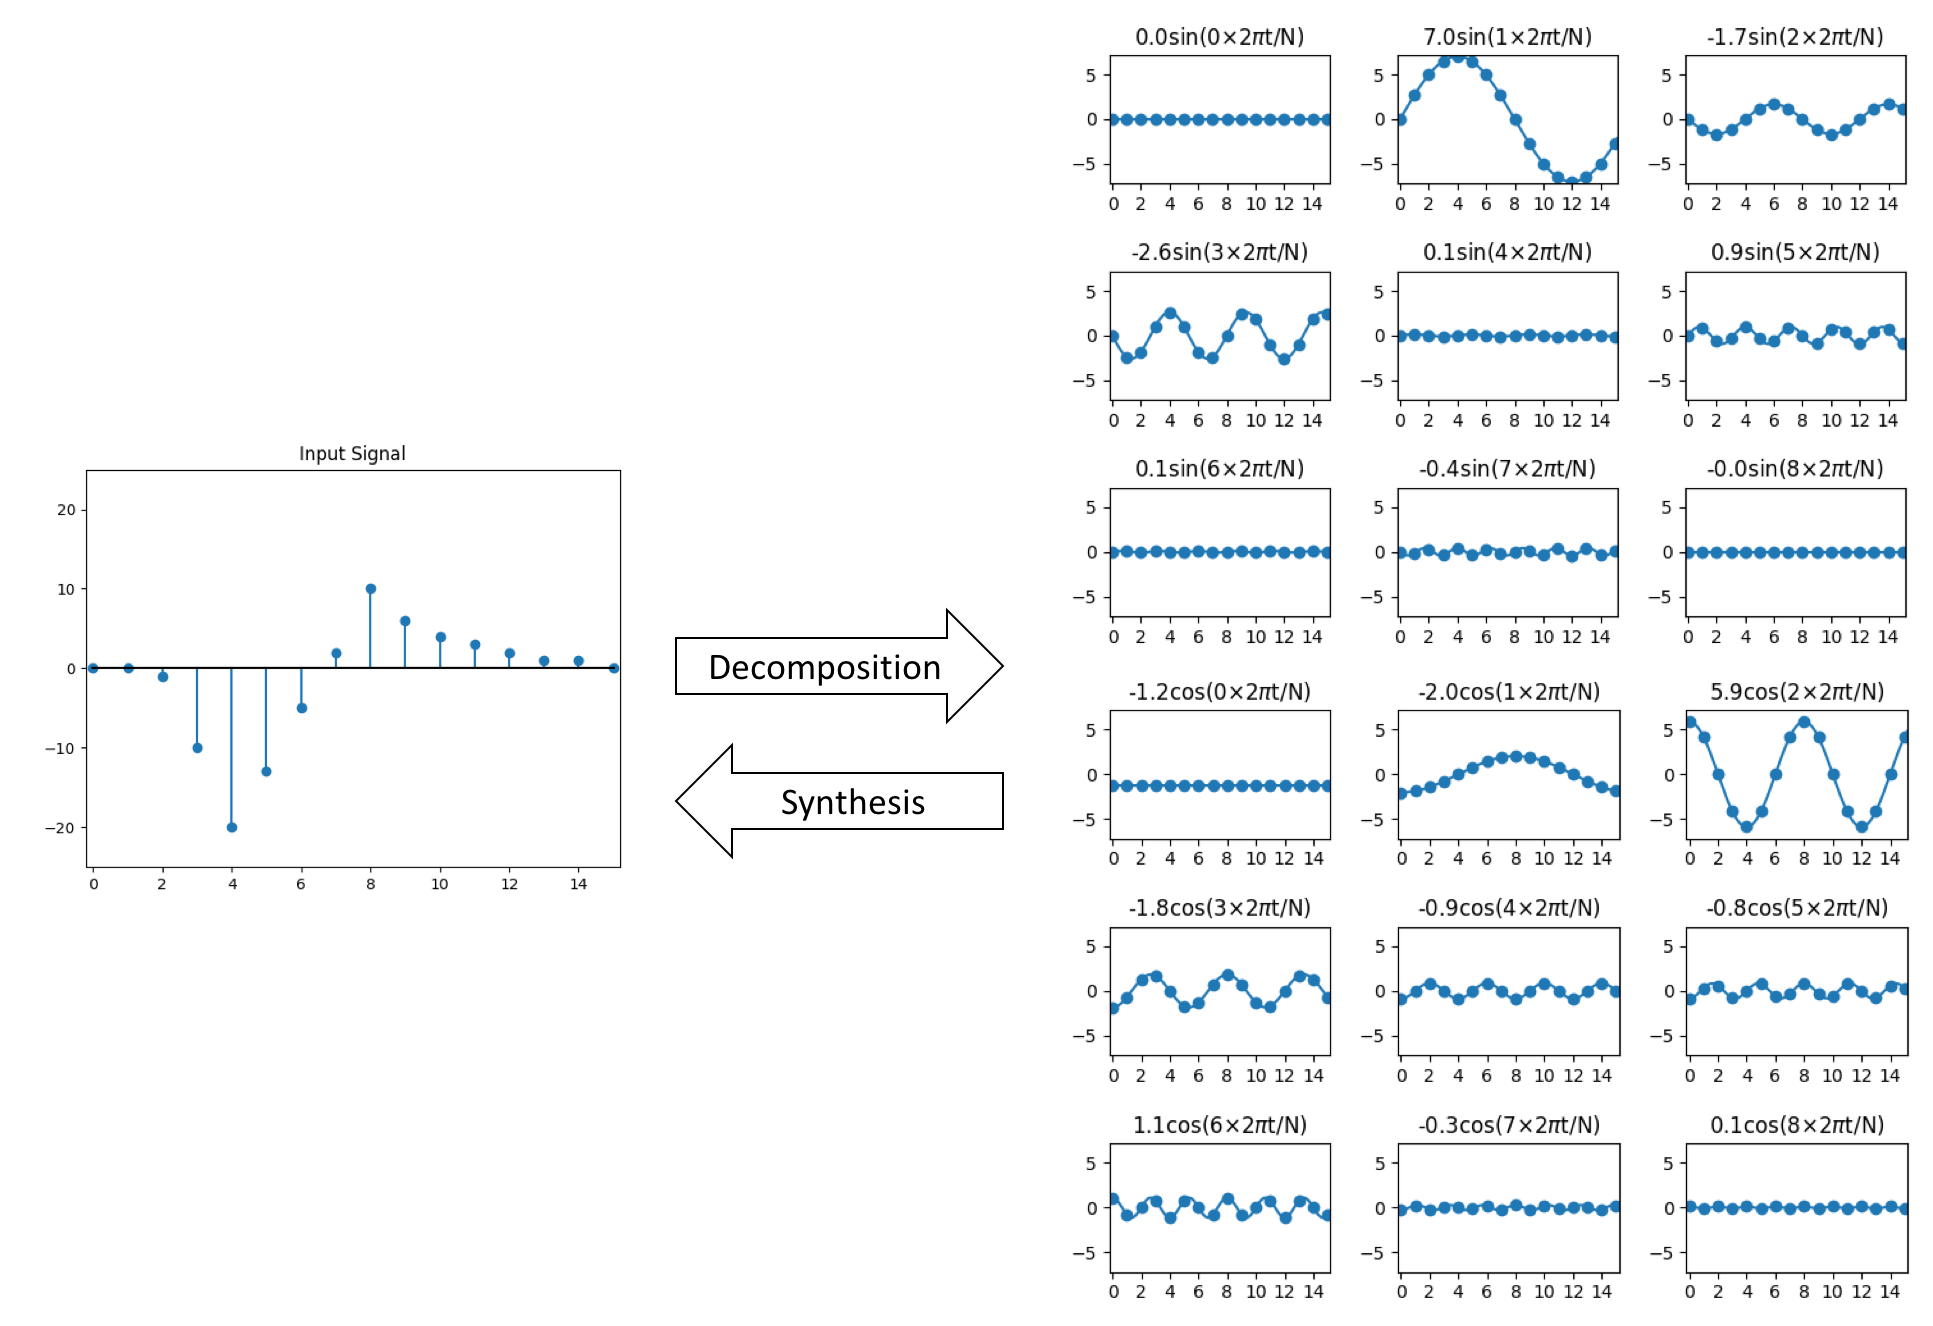
\includegraphics[width=\textwidth]{_images/DecompSynth.png}
\caption{\textbf{ Decomposition-Synthesis Relationship |} A comparison between an input signal (left) and the 18 sinusoids (right) which can be used to reconstruct the original sequence. Generally, we say that the input image can be decomposed into the 18 signals on the right and similarly that the 18 signals can be used to synthesize the original signal. 
}\label{fig:deco}
\end{figure}

\begin{figure}
\centering
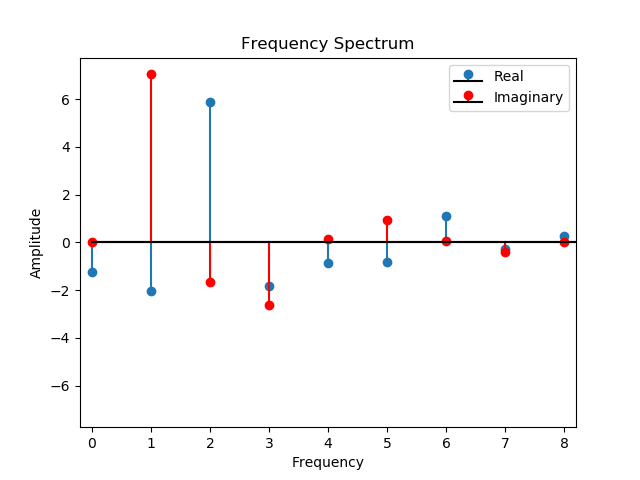
\includegraphics[width=\textwidth]{_images/FreqSpec.png}
\caption{\textbf{Frequency Spectrum |} In Figure \ref{fig:deco}, we decomposed a signal into 18 sines and cosines with different frequencies and amplitudes. The frequencies of these sinusoids are predetermined by the length of the input signal and the amplitudes are determined by the Fourier transform. 
}
\end{figure}



\begin{figure}
\centering
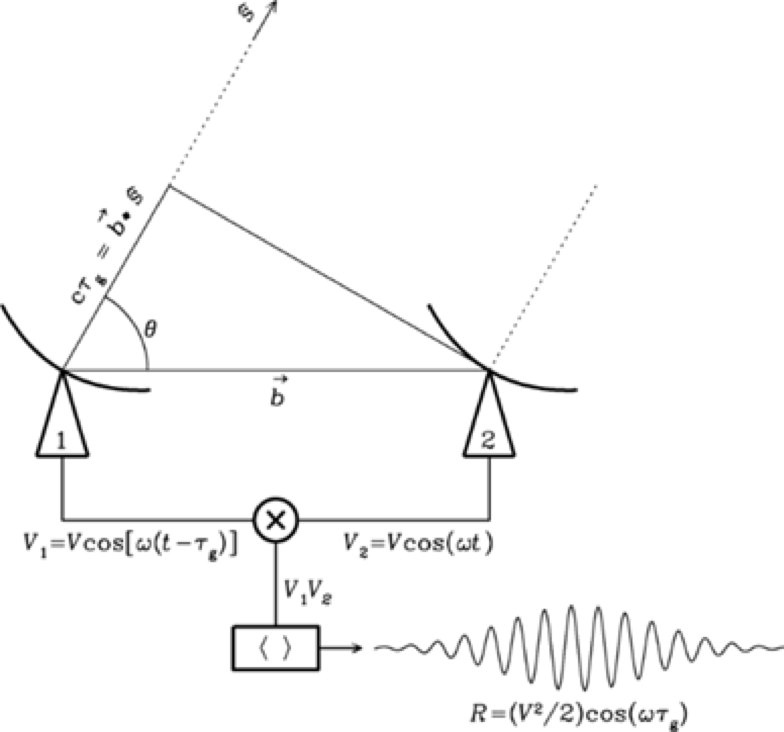
\includegraphics[width=.8\textwidth]{_images/AntGeometry.png}
\caption{\textbf{Fringe Pattern Analysis |} Schematic shows that two antennas separated by a distance $\vec{b}$ will receive time delayed versions of the same ``galactic'' signal, $V\cos(\omega t)$. If we then multiply these signals and average them over period of time, then we will obtain a signal, R, which depends on the direction of the source, $\hat{s}$, through $\tau_g$ since $\tau_g = \vec{b} \cdot \hat{s} / c$.
}
\end{figure}


\begin{figure}
\centering
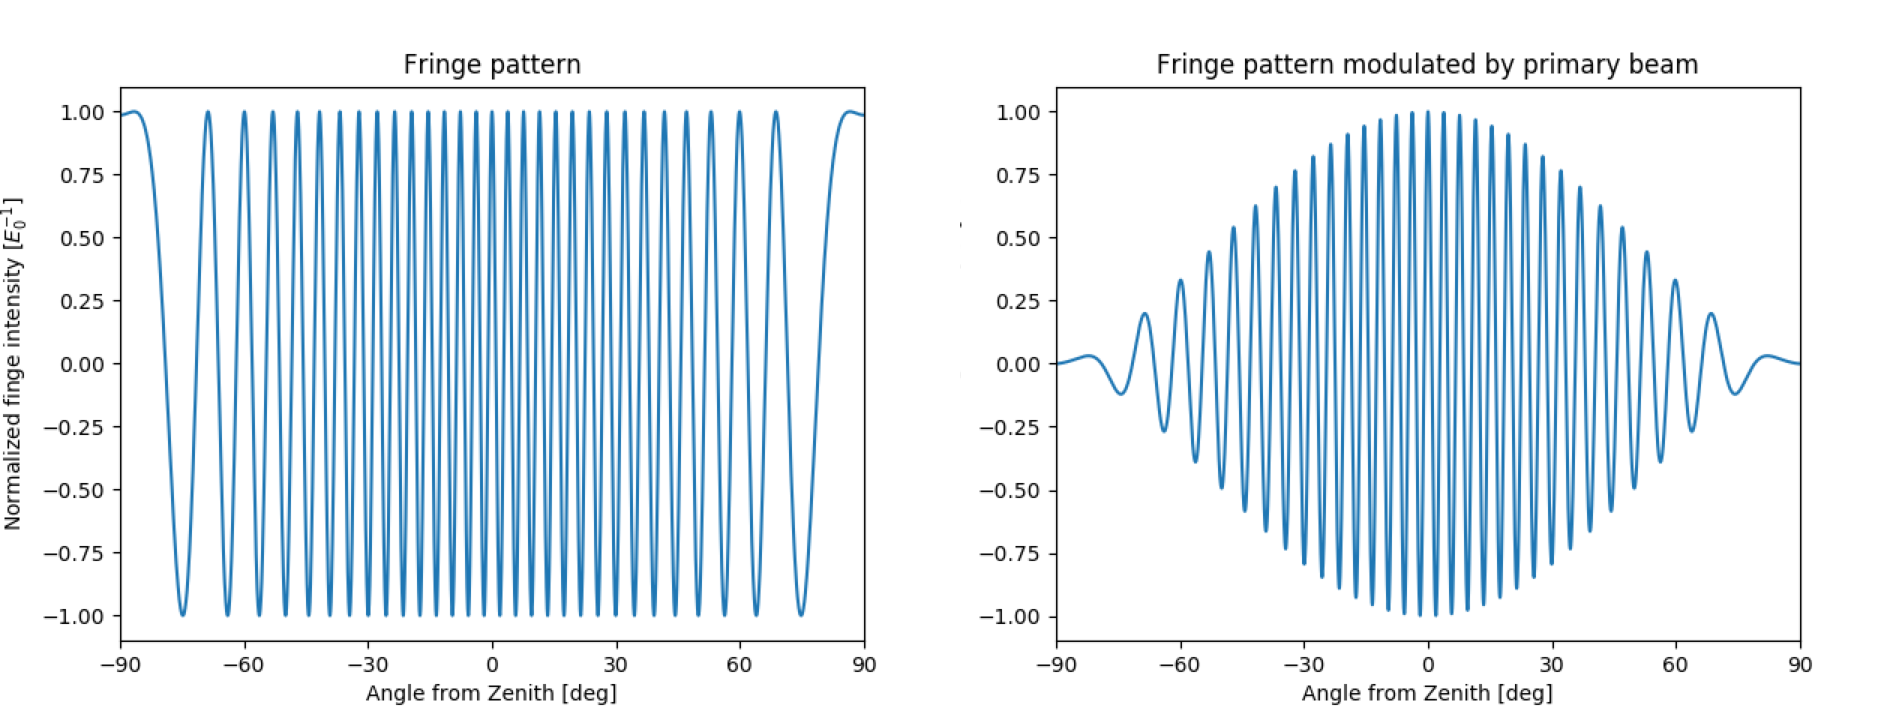
\includegraphics[width=\textwidth]{_images/FringePattern.png}
\caption{\textbf{ Idealized Fringe Pattern |} Fringe patterns for a pair of hypothetical omni-directional antennas. Fringe patterns can be thought of as directional sensitivity patterns that describe how effectively radiation from any given direction will be picked up by the antenna.}
\end{figure}



\end{document}